% !TeX root = paper.tex
\documentclass[a4paper,12pt]{article}

% Packages
\usepackage[utf8]{inputenc}     
\usepackage{amsmath, amssymb} 
\usepackage{graphicx}          
\usepackage{geometry}           
\usepackage[numbers]{natbib}            
\usepackage{hyperref}          
\usepackage{subcaption}         
% Page layout
\geometry{margin=1in}          

% Title section
\title{TIM: Tree Imaging Machine} %emw24Feb: Do we need a better title for the paper? LIke: TIM: A Tree Imaging Machine for low-cost digital images of tree cores and cookies ?
\author{Your Name}
\date{\today}




\begin{document}

\maketitle

%emw24Feb: I added some text to abstract and intro that I am not 100% sure you would need for some journals, but I think you will need for MEE. 
%emw24Feb: I was trying to add this tag '%emw24Feb:' to my comments, but got lazy and just added them below without the tag generally. Please delete my comments in the tex once you have dealt with them!

\begin{abstract} 
Studies of tree rings (dendrochronology) have benefitted recently from new methods to image wood rapidly and efficiently, helping to scale up the number and quality of image samples. Current open-source approaches are, however, limited in dimensionality and can be cost-prohibitive. The Tree Imaging Machine (TIM) is a do-it-yourself scanning tool made to digitize tree cookies and cores that address these limitations. TIM takes partially overlapping microscopic images of samples and stitches the individual images together to form 
a mosaic, which can be zoomed in to visualize features on the scale of 0.01 mm. With scans of up to 21 140 DPI, TIM produces one of the highest resolution images among similar tools for the competitive price of less than \$3 000 USD.
We designed TIM to have a large working plane to allow digitizing individual cores over 50 cm and to allow the operator to set a batch of samples to digitize without operator intervention.  %emw24Feb: Could we say operator assistance? Or just: without any help from the operator? I also don't totally get what we mean here ... what are a batch of samples? Do we mean cores or multiple cookies? I might rephrase as: We designed TIM to have a large working plane to allow digitizing individual cores over 50 cm and batch sampling. With batch sampling ... 
All of the 3D printed parts are available for download on the NIH 3D printing repository (ADD LINK or reference?) and the software is 
open source, with instructions to recreate this tool available at (ADD LINK). TIM provides an important advance in (resolution, cost, functionality, all-in-one package?) that advances tree ring sampling to tackle larger samples and collect data at finer resolutions in an open-source design that can be built on and improved as new technologies become available. % Add to the discussion something about next steps for TIM more clearly? 
\end{abstract}

\section{Introduction}
%emw24Feb -- move around and add cites below to fit with current text. You should cite a Michael Mann paper, such as Proxy-based reconstructions of hemispheric and global surface temperature variations over the past two millennia
Multiple fields---from climatology to forestry and ecology---rely on tree rings to understand how the environment affects tree growth. Tree rings have been critical to 
reconstructing past climates of regional and local environments, informing our understanding of climate change today \citep{fritts_dendroclimatology_1971} \citep{williams_using_2010} \citep{guibal_dendrochronology_2021} \citep{sheppard_dendroclimatology_2010}. They are also increasingly used in ecology,  to understand how plant competition affects tree growth in addition to climate % cite https://besjournals.onlinelibrary.wiley.com/doi/full/10.1111/1365-2745.12782
and with implications in forestry to managing stand dynamics. % maybe cite https://cdnsciencepub.com/doi/abs/10.1139/x03-232?casa_token=tzQCqy0zaGwAAAAA:5b-e-8-9OT4MZ_rxgxr4KrD7oXZ4KCcZi0S-e7ZaGCMB_gUfC8n_b4DcYuda5GT8DStxnWpA8BY7_A
As tree growth and forest management becomes more critical to mitigating climate change, scaling up the collection and processing of tree ring samples has become increasingly important. 

%One of many examples of removing PV 
% You should ask Mao for the tree ring methods book ref and define these things quickly then cite it. 
Data from the tree rings comes from measured tree rings widths from a tree cookie (DEFINE) or core (DEFINE). The first high precision tool for this purpose was a stage micrometer, which requires a trained technician to incrementally shift a tree core under the objective of a microscope---informing an attached computer when a new ring is encountered \citep{robinson_microcomputer_nodate}. % How does the 'informing' happen? I think you could make this more informative and use active voice ... do they click something or what? 
While this method has very high precision, the data are only as accurate as the experience and knowledge of the technician at the time of recording as no permanent image record is produced \citep{levanic_atrics_2007}. 

Image analysis of tree rings was designed to reduce both errors in sampling and sampling bias across individual technicians, with major methods developed in (late 1980s to 1990? And add cites) to digitize tree ring samples using flatbed scanners. Early techniques used a flatbed scanner to digitize the entire sample at once \citep{guay_new_1992}, producing maximum resolutions of 4800 dpi and scan an area of up to  21.6 cm x 29.7 cm (e.g., using a top of the line scanner, like the Epson Perfection V850 Pro) % I think we can skip inches .... 8.5 inches x 11.7 inches
More recent techniques have aimed to achieve higher resolutions and/or larger samples through a different digitization approach, called ATRICS \citep{levanic_atrics_2007}. % Should we spell out ATRICS? Also I think we should introduce the METHOD, then say ATRICS is an example of it (for example, 'through a different digitization approach, which takes multiple images then stitches them together. One widely used version of this was ATRICS ...'), but I am not sure if that is true so will take a look on next version; feel free to add info here in the comments. 
Rather than scanning a whole sample at once, with ATRICS a high resolution camera takes multiple images across the surface of the sample then uses image stitching software to combine them into one ultra high resolution image \citep{muhlich_stitching_2022}.
Stitching multiple images into one mosaic has been applied in other fields such as mineralogy and cellular biology \citep{ro_image_2021,mohammadi_fast_2024}. 
This method requires either the camera objective to move relative to the sample, or the sample move underneath a stationary camera. 

% I would start a new paragraph here that opens with something like: Since XX was introduced in XX, image capture and stitching of tree rings has increased. Today CaptuRING offers a  more modern do-it-yourself alternative to ATRICS that is (open source? Has resolutions up to XX? Used XX type of camera? Give a little more here). Another approach, Gigapixel, moves the camera relative to the sample, allowing for multiple samples to be recorded in sequence \citep{griffin_gigapixel_2021}. 
% Then I would end on the cookies issue and also anything else to mention, like cost? You should also clearly mention when/how stitching happens in these approaches.
For ATRICS and a more modern do-it-yourself alternative, CaptuRING, the sample is moved relative to the camera \citep{garcia-hidalgo_capturing_2022}. 
Gigapixel takes a different approach by moving the camera relative to the sample, allowing for multiple samples to be recorded in sequence \citep{griffin_gigapixel_2021}. 
While these machines can all digitize cores, none have been shown to digitize cookies. % I think you could build up to this point by adding in that the above approaches move in one linear direction or such? 

% I will edit this a little next time, but for now fix up em-dashes, and simplify with less PV as possible. 
TIM was made to combine the defining features of the previously mentioned machines into one while making the project open-source and open-hardware. 
We designed TIM to digitize both cookies and cores, increase the maximum sample length, perform image stitching without operator intervention, and capture batches of samples in a queue - all while minimizing cost. 
The only specialized piece of equipment needed to build TIM is a 3D printer, but the parts can be readily ordered through 3D print shops if preferred.
Excluding 3D printed parts, the total cost of the machine is approximately \$2 200 USD compared to the \$70 000 USD of the Gigapixel \citep{griffin_gigapixel_2021}.
The total cost of the machine is almost comparable in price or less to many professional camera and macro lens combinations.
Additional savings can also be had when factoring in the cost of a professional stitching software license such as PTGui. 

\section{Methods}

\subsection{System Overview} % this is so dry fix later
% Can we have an a photo as a figure that we link to here? 

% Good topic sentence! Can you walk reader more carefully through each item? You may need to re-order them .. But basically, pick the most useful order and then write: For the camera .... For the gantry machine ... You might also use this space to say, in contrast to previous approaches that have used XX giant camera, we used ... and otherwise point out the novelty when it comes up. 
TIM can be thought of as a combination of multiple subsystems: the camera, computer, and gantry machine. 
Cartesian movement in the X, Y and Z directions is a result of two machine kits and a motor controller from OpenBuilds - the ACRO 1010, the NEMA 17 lead screw linear actuator, and the X32 Motor Controller running GRBL firmware. 
Smaller and larger working planes easily be achieved by purchasing a different sized ACRO kit.
Building on top of kits allowed for quick assembly with sound instructions and saved development time. 
To fit on the build plates of the ACRO system, we made an adapter to connect the linear actuator to the X and Y axis, thus creating motion in the Z axis.
On the linear actuator's build plate, adapters were made to hold a 12MP Raspberry Pi HQ Camera equipped with a SEEED studio microscope lens connected to an NVIDIA Jetson Orin Nano (Jetson) through a CSI cable.
% Nice active voice below!
By choosing this combination, we were able to reduce the weight and cost of the camera significantly, which allowed us to invest more in an efficient computer that can handle intensive image processing. 
The Jetson is a powerful edge computer which drives a monitor for a GUI, sends commands to the motor controller to move the machine, runs image processing calculations for automatic control, and performs calculations to stitch individual images into one mosaic. 
Despite the weight reductions, torsion on the gantry arm still resulted in a non-zero torsional deflection. A torsion correcting adapter was designed to counteract this rotation and level the lens.


\subsection{Preparing Cookies and Cores}
% Tried to reduce PV below. 
TIM can scan both tree cookies and tree cores. Sample preparation for both are equally important but require different approaches.
Similar to general sample preparation methods for tree rings samples (CITE dendro manual), cookies and cores need to be sanded with incrementally increasing sand paper grit to produce an even surface for scanning. We sanded cookies using an orbital sander with mesh sandpaper from 60 to 800 grit, then used a microscope to visually inspect the quality of the sanding. We considered the sample to be sufficiently prepared when vessels were easily identifiable.

Special sanding considerations need to be taken for each sample type. 
For cookies, it is important to have the top and bottom surfaces be nearly parallel. Small differences in plane angle can be corrected using the 3D printed levelling table we designed (See Figure \ref{fig:ideal_levelling}). 
For cores, care should be taken to maximize the scanning surface. This means removing material to be coincident to the center of the cross section of the core. 
Similarly to cookies, care should be given to achieving a  scanning surface as parallel to the XY-plane as possible.
Cores also need to be aligned to be parallel to the Y axis to be digitized, using squaring tool or similar to help with alignment. Any warping in core mounts need to be counteracted with the use of trigger clamps. 

\subsection{Sample Digitization} % Methods
% It would be super nice to have a concept image of this process! 
The subsystems of TIM can be best understood by following the process from sample setup through through obtaining a stitched image. 
To achieve this with a fixed focus camera, the samples must be nearly orthogonal to the camera lens. 
Once the sample is level, the operator interacts with the machine through the GUI to navigate the camera to the center of the sample, and focuses the preview image to be sharp by moving in the Z axis. The height and width dimensions are then entered in the GUI
to be saved along with the detected center coordinate of the sample. This procedure can be repeated to create a queue of samples to digitize as a batch.
The height, width, identifiers, sample type, and centering of the sample is sufficient information to digitize.

\begin{figure}
    \centering
    \begin{subfigure}{.5\textwidth}
      \centering
      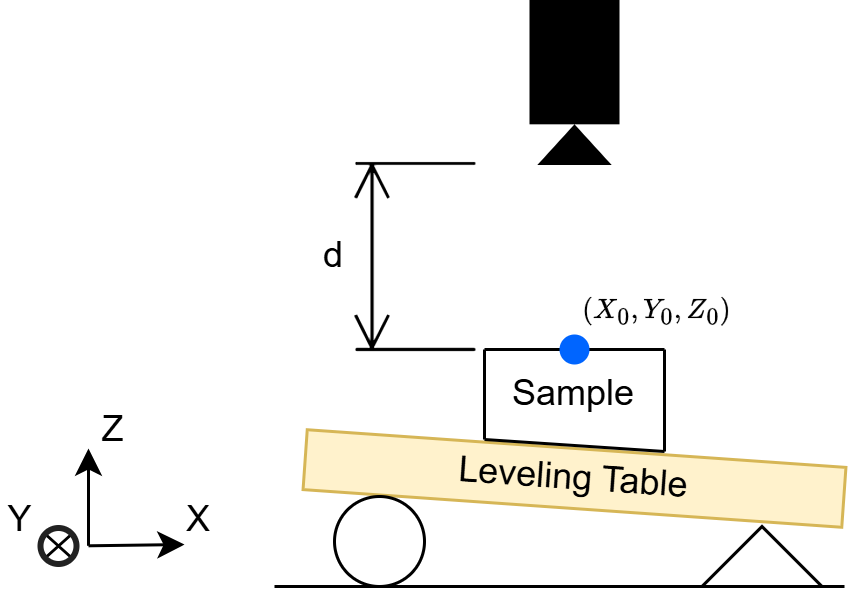
\includegraphics[height=0.5\linewidth]{../diagrams/sample_setup_ideal.png}
      \caption{Ideal sample leveling}
      \label{fig:ideal_levelling}
    \end{subfigure}%
    \begin{subfigure}{.5\textwidth}
      \centering
      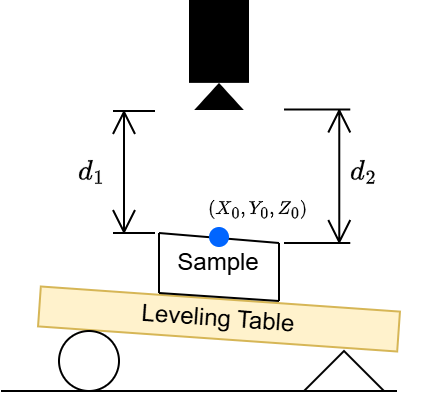
\includegraphics[height=0.5\linewidth]{../diagrams/sample_setup_realistic.png}
      \caption{Realistic sample leveling}
      \label{fig:realistic_levelling}
    \end{subfigure}
    \caption{Side view of the camera and sample on top of a leveling table. The ideal sample leveling shows a uniform distance d at all $(X,Y)$ coordinates on the sample. This is impossible to achieve in reality, the true sample leveling has a non uniform distance at unique $(X_i, Y_i)$.}
    \label{fig:sample_levelling}
\end{figure}


\subsection{Image Capturing} % Could this be Image Capture? 
In the GUI the operator indicates the height and width of the field of view in an individual image from the camera. 
This varies on the focal length of the lens, but we have kept the field of view to be 3mm x 5mm. 
Once prompted the system begins to exhaustively traverse the surface area of the sample, using the sample height and width entered by the operator.  
The goal of this traversal is to obtain in-focus images that have a region of overlap with all its neighbors - the basis of image stitching. 
Digitizing cores can be done without needing to traverse in both the X and Y axis. 
The optimal scanning path for a core is to ignore the Y axis and traverse the cores length.
Spanning the surface area of a cookie requires movement in both the X and Y axis.

% I am not sure what 'implement automatic control to focus the images' ... I started an improved sentence below, but stalled because I am not sure what you mean.... 
% Centering the design of TIM around a fixed focus camera and lens means we need to automatically focus the images.
By centering the design around a fixed focus camera and lens, it is necessary to implement automatic control to focus the images. 
The only way to control the focus of a fixed focus lens is by changing the lens's distance to the sample. 
And with the microscope lens, the depth of field of the image is so sensitive that sub millimeter heights can move an entire image out of focus.
Solving this in a time-efficient manner involves two stages. 
The first stage takes advantage of the requirement to navigate and focus the camera to the center of the sample.
This allows the initial $Z_0$ value, captured when adding a sample, to be an informed guess as to what value would have an in focus image across the entire surface. 
From the first $(X_0, Y_0)$ coordinate captured, 11 images are taken at different $Z$ values in $\boldsymbol{Z_{\text{samples}}}$. 
So long as $Z_{focused}$ is within this set, an in focus image exists. % why 11? 

% Something bad is happening with the i below. 
\[
Z_{focused} \in
\boldsymbol{Z_{\text{samples}}} = 
Z_0 + 
\begin{bmatrix}
-0.5 \\
-0.4 \\
\vdots \\
0.4 \\
0.5 \\
\end{bmatrix}
% \exists 
% Z_{focused}
\] % unsure if this makes sense

Our focusing procedure begins at 0.5 mm above $Z_0$ and finishes with the last image at 0.5 mm below $Z_0$.
The 11 images then have their normalized variance, $NV$, calculated in a separate thread to measure the image sharpness \citep{sampat_extensive_2014}.
The image with the maximum score is saved and can be considered the most in focus image, while the rest are deleted from storage.

\[
  i_{\max} = \arg\max_{i} NV(image(\boldsymbol{{Z_\text{focus}})})
  \]

This focusing procedure works well alone when the sample alignment has a difference in height no greater than 0.5 mm, $d_1 - d_2 < 0.5 mm $ (See Figure \ref{fig:realistic_levelling}). 
% And while 1mm may sound like a small range, it is important to note that increases in time at each $(X_k, Y_k)$ are repeated $k$ times. 
Rather than adjusting this range, a greater alignment error can be managed by controlling the center of the range, $Z_{0,k}$, for $(X_k,Y_k)$. 
The likelihood of an adjacent $(X_{k+1}, Y_{k+1})$ containing an in focus image is highest when the current $i_{{\max,k}}$ is at the middle index of $\boldsymbol{Z_{samples}}$. 
A PID control algorithm with a process variable of $i_{max}$ and control variable of $Z_{0,k}$ allows a negative feedback loop to improve focusing across the entire sample \citep{odwyer_summary_2000}. 
Instead of $(Z_{max} - Z_{min}) < 0.5mm$, now the system can handle $(Z_{k} - Z_{k+1} < 0.5mm)$ which allows for a more forgiving sample setup. After the capturing overlapping images across the entire surface area, the images are ready to be stitched.

To reduce motion blur in the images, the range of $\boldsymbol{Z_{\text{samples}}}$ is traversed at constant velocity and images are captured without stopping. 
Decoupling the auxiliary camera control from the G-code commands to control the machine has shown to improve speed and decrease vibrational effects from acceleration and deceleration \citep{propst_time_2025}.
This is a variation of the standard approach used in 3D printing and CNC control methods. % What is CNC? 
  
\subsection{Accounting for Translation Error Between Core Samples}

Difficulties arise when more than one core are added to the digitization queue.
The ACRO has a theoretical 4.5 micron translational accuracy, but is hard to achieve.
These inaccuracies can cause drift in the images with relation to the core and result in the width of the core not being within the field of view of the images.
We thus implemented a centering procedure that realigns the center of the core to the center of the image frame when the machine moves 
to a new sample. 

First, the camera is moved to the $(X_0, Y_0, Z_0)$ of the new core. 
From there, the camera is moved across a window, at constant velocity, from $(X_0 - 1/2*{range}, Y_0, Z_0)$ to $(X_0 + 1/2*{range}, Y_0, Z_0)$. 
Images are captured at equal distance intervals analogously to the image focusing procedure. 
Once again, the image with the highest normalized variance score is considered the best image and its location is used as the realigned $X_0^\prime$.
This procedure drastically improves digitization quality of batches of cores.

\subsection{Stitching}

Image stitching is a well explored field, ranging from panoramic images taken on smart phones to highly tuned microscopy slide stitching. 
But the basis of stitching remains the same across algorithms. Adjacent images must have a region of overlap. 
Of the stitching tools with a software API that we tested, only the Python package Stitch2D was able to stitch our images successfully into a grid. % need to reference this
This package wraps OpenCV functions for finding distinctive image features using the SIFT feature detector and matches these feature within the overlapping region of adjacent images \citep{lowe_distinctive_2004}. 
The default implementation of the package works very well but has an $O(2n)$ space complexity and fails due to out-of-memory errors when stitching hundreds of images. %is this wording correct?, I'm trying to kindly say it was memory inefficient
With a few key memory conscious changes to the algorithm, the space complexity was reduced to approximately $O(\log{n})$ and the package was able to run on the Jetson without a problem. 

% What do we mean below? I think we might need to use more words (and sentences) to spell this out for readers: Some tree ring projects/analuses may not need high resolution images and could be needlessly slowed by TIM's approach ... 
Depending on the analysis, it is unnecessary to digitize samples at a very high DPI. To address this, a parameter in the machine configuration file 
allows the user to downsize images before they get stitched together to avoid unnecessary sample detail and decrease the size of the files.
With the same images, multiple final stitched resolutions can be made. 

\section{Results}

\begin{figure}
  \centering
  \begin{subfigure}{.5\textwidth}
    \centering
    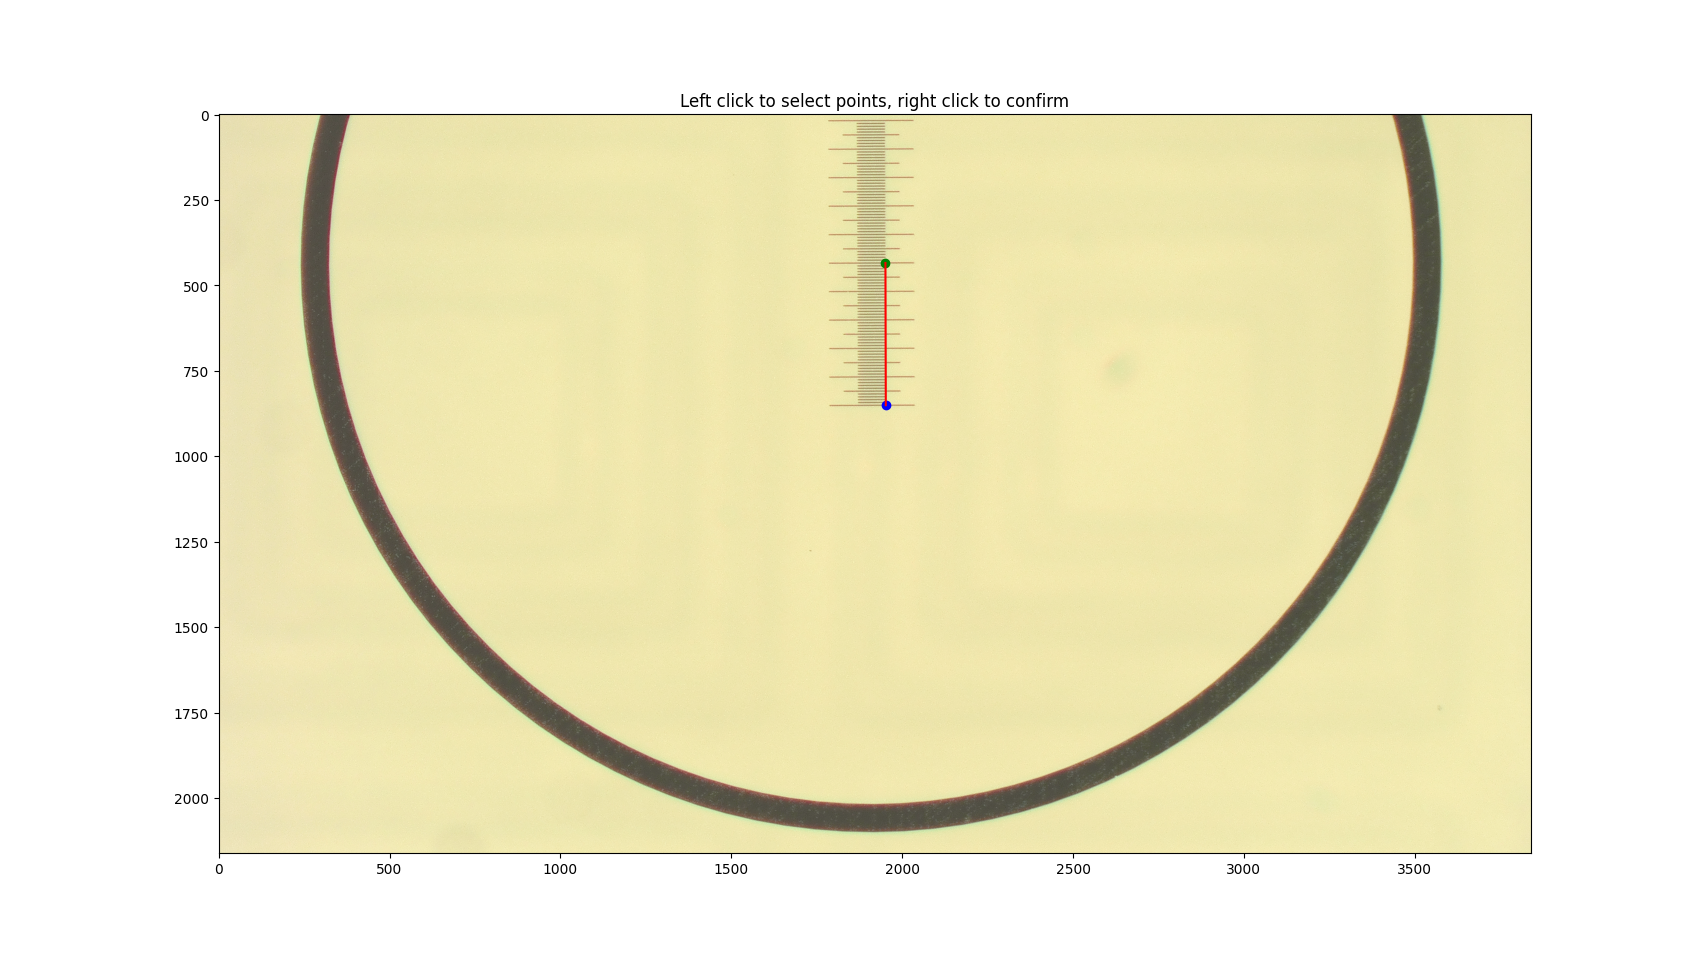
\includegraphics[height=0.5\linewidth]{../diagrams/dpi_measurement_whole.png}
    \caption{Scale Bar for DPI measurements}
    \label{fig:dpi_measurement_whole}
  \end{subfigure}%
  \begin{subfigure}{.5\textwidth}
    \centering
    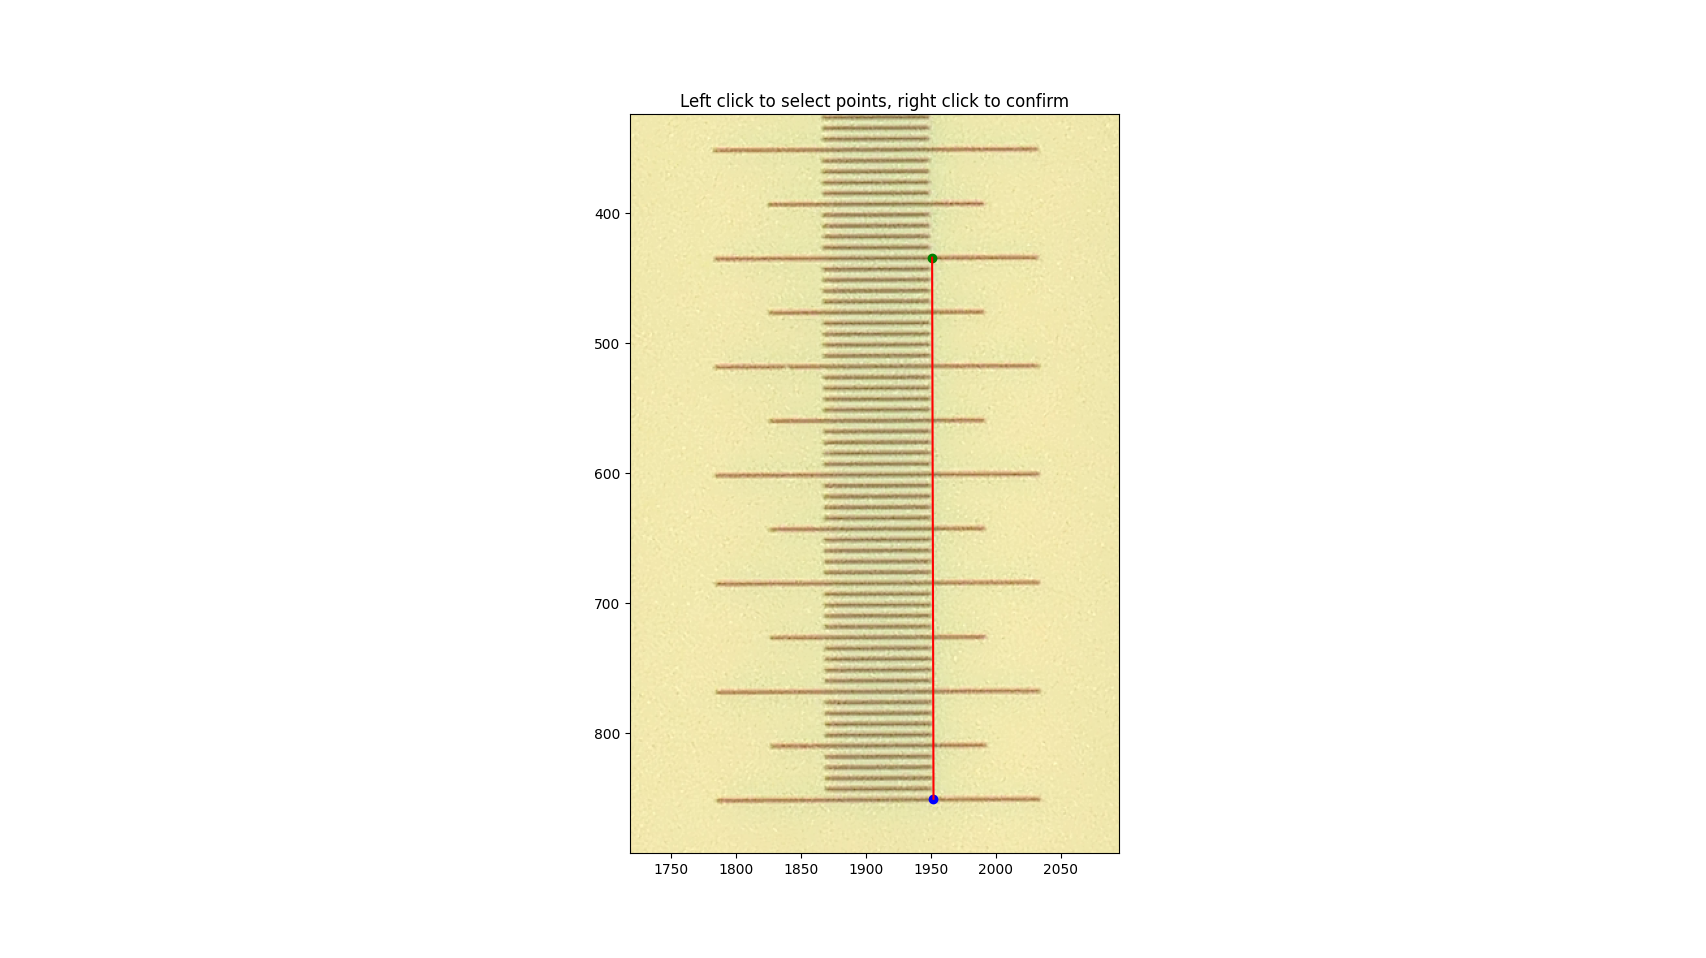
\includegraphics[height=0.5\linewidth]{../diagrams/dpi_measurement_zoomed_2.png}
    \caption{Zoomed in Scale Bar}
    \label{fig:dpi_measurement_zoomed}
  \end{subfigure}
  \caption{Example of a single DPI measurement using a 0.01mm slide scale. The DPI was measured at multiple locations in the field of view both vertically and horizontally. They converged on the same value.}
  \label{fig:dpi_measurements}
\end{figure}

TIM is capable of producing extremely high resolution scans.
A microscopy slide scale with 0.01mm graduations was used to calculate the dots per inch (DPI) of individual images captured from the system (Figure \ref{fig:dpi_measurements}).  
Using this scale we calculated the maximum DPI to be 21,140. This calculation can be replicated using the Python tool we created as necessary for varied lens focal lengths. When downscaling the final stitch, 
DPI scales linearly with the downscale percentage defined in the machine parameters. 

TIM has been used to digitize 90 cookies and is in the process of finishing 1,200 cores. % I would move this to the end of the results and/or just put it in the cover letter to the journal. 

Digitizing samples takes significantly longer for cookies than it does for cores (Figure \ref{fig:digitization_time}). This is due to the surface area of cookies requiring more images as it has a square relationship to sample radius.
For large cookies, the operator can choose to selectively scan a portion of the cookie. Scanning cookies at maximum resolution is unrealistic as the max cookie size is very small. 
To fit into the maximum 2.5 GB limits of a TIFF file, the maximum diameter of a cookie scanned at 30\% of maximum resolution is limited to approximately 130 mm. For cores at maximum resolution, this file size limit 
constrains samples to approximately 1,500 mm in length. Note that a larger ACRO frame would be needed to support this sample length. Samples that are larger than this file size limit are still possible to be scanned but they are no longer stored as a TIFF file. 
An uncompressed binary NumPy memory-mapped array file is produced. This implies that the operator knows how to splice into these files and is comfortable working with NumPy memory-mapped arrays in Python.

\begin{figure}
    \centering
    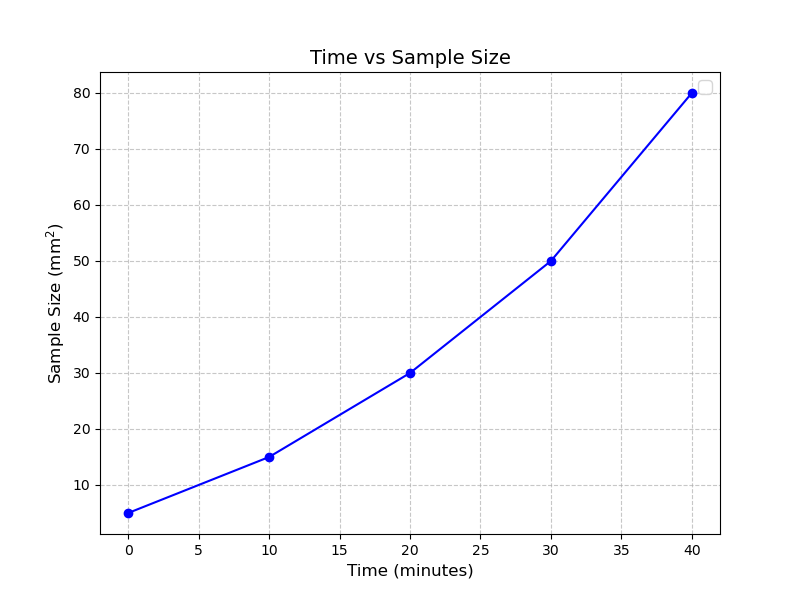
\includegraphics[height=0.5\linewidth]{../../code/plots/time_and_area.png}
    \caption{Time to digitize a sample is dependent on the sample's surface area and the desired final resolution.
    Cores benefit from linear surface area to sample length. The range of sample included are from a 3mm x 220mm core to a 75mm x 56mm cookie. True sampling times are drastically influenced by configurable machine parameters.} % Take the title on top off this image as we don't have titles on images in sci papers. 
    \label{fig:digitization_time}
\end{figure}

\section{Discussion} % I think we could remind the reader here of what gaps TIM addresses, but I can help do that next time. 
By taking advantage of a common three degree of freedom cartesian machine design, powerful edge computing, and a microscope camera we were able to design a cost effective and high resolution digitization tool for wood samples. 
We significantly increased the maximum sample length and maximum resolution compared to common alternatives in the field. 
In addition, the machine design was intended to be readily replicated by labs with minimal engineering experience and equipment. 

\subsection{Strengths and Opportunities}
% Try to reduce PV here please!
Our design has tried to minimize the barriers to building this machine in smaller labs. After investing a few hours in the sourcing and assembly of parts, 
the rest of the implementation has been completed. Digitized samples from this machine have been able to have tree rings registered onto their images using CooRecorder.
Integration into a cloud data storage system would be a great addition to remove the need for an operator to move the final data with a physical external drive. 
Further testing with vessel counting models or ring identification models would be an interesting extension to take advantage of high resolution scans. % I guess Sandy never sent in results we could use? 

\bibliographystyle{plainnat}
\bibliography{references}

\end{document}
